%\documentclass[../../Orator]{subfiles}
\documentclass[class={myRUCProject}, crop=false]{standalone}
\IfStandalone{%
  \import{../../}{customCommands}
  \import{../../}{INP-00-glossary}
  }{}

\usepackage[subpreambles = true]{standalone}
\usepackage{myTikz}


\begin{document}


\begin{figure}[H]
  \centering
  \import{../../Pictures/Anakin}{Neuron.tex}
  \caption{A simplified representation of a \gls{gls:neuron}[al] cell, with labels for each of the important features. (1) the \gls{gls:soma} of the cell; (2) a \gls{gls:dendrite}; (3) the \gls{gls:axon}; (4) the \gls{gls:ax-hill}; (5) the \gls{gls:ax-terminal}.}\label{fig:Neuron}
\end{figure}

The human body is composed of a vast number of cells and complex interactions, how could anyone ever expect these meaty lumps we call `\textit{\glspl{gls:person}}' to coordinate properly without an equally complex system for the transfer of information? 
\Glspl{gls:neuron} are information highways made manifest in multi-cellular organisms. 
There exist many distinct types of \glspl{gls:neuron}, however, the underlying mechanisms of function stay the same.

\section{Cellular Structures}
\subsection{Organelles}
\begin{enumerate}

  \item \textbf{The Nucleus} is mainly found in the centre of the cell and is responsible for distinguishing between eukaryotic and prokaryotic cells - existing only in the first ones. It functions as the key factor in the cell's activities, it contains the cell's genetic information (DNA), and is where the DNA replication, transcription, and RNA processing all happen.
  \item \textbf{The Ribosomes} exist both in eukaryotic and prokaryotic cells. By translating the genetic information from the RNA, they compose proteins and convert genetic code into chains of amino acids.
  \item \textbf{The Golgi-Apparatus}, an organelle mostly found in eukaryotic cells, transports, modifies, and packages proteins and lipids into vesicles destined for specific intracellular or extracellular locations.
  \item \textbf{The Endoplasmic Reticulum (ER)} is a cellular organelle that also plays a crutial role in protein and lipid synthesis. There are two types of ER; the rough and the smooth. Rough ER is composed of ribosommes, giving it its rough texture. In contrast, smooth ER gets its smooth surface because of the lack of ribosomes.
  \item \textbf{The Lysosome} is covered by a membrane and consists of digestive enzymes. Their role is to break down cell parts and eliminate invading viruses and bacteria.
  
\end{enumerate}

\subsection{Specialized Neuronal Structures}
There exist a number of important features that are foundational to the specialized functions found in the \glspl{gls:neuron};
\begin{enumerate}
  \item \glslink{gls:soma}{\textbf{The soma}} is the main body of the \gls{gls:neuron}. It is the space in which the nucleus resides, and by extension where protein production occurs. The nucleus can range from \qtyrange{3}{18}{\um} in diameter.
  \item \glslink{gls:dendrite}{\textbf{The dendrites}} of a \gls{gls:neuron} are extensions of the \gls{gls:membrane} with many branches. This overall shape and structure are metaphorically referred to as a `\textit{\gls{gls:denTree}}'.\footnotemark This is where the majority of \gls{gls:neuron} inputs are received, and carried by the `dendritic spine' down to the \gls{gls:soma}~\cite{}. \footnotetext{Greek root word `\textit{dendron}' meaning tree, translates to `tree tree'.}
  \item \glslink{gls:axon}{\textbf{The axon}} is a finer tendril that can extend tens, if not tens of thousands of times, the diameter of the \gls{gls:soma} in length. The \gls{gls:axon} primarily carries nerve signals away from the \gls{gls:soma} and carries some types of information back to it. Most \glspl{gls:neuron} have only one \gls{gls:axon}, but this \gls{gls:axon} will be able to undergo significant branching, enabling communication with many target cells. 
  \item \glslink{gls:ax-hill}{\textbf{The axon hill-lock}} is the part of the \gls{gls:axon} where it emerges from the \gls{gls:soma}. The region contains the greatest density of voltage-dependent sodium channels. This makes it the most easily excited part of the \gls{gls:neuron}~\cite{}. 
  \item \glslink{gls:ax-terminal}{\textbf{The axon terminal}} is found at the terminus of the \gls{gls:axon} and contains synapses. 
  \item \glslink{gls:myelin}{\textbf{The myelin sheathe}} is a lipid and protein comprised substance excreted from ??? cells that `sheathes' the \gls{gls:axon}, creating additional insulation for \gls{gls:capa}~\cite{}.
\end{enumerate}


\section{The Resting Membrane Potential} 
A fundamental component of cells is the \gls{gls:membrane}, composed of what is known as a `\gls{gls:bilipid}'.{}\footnote{Latin root word `bi' meaning two, translates to `lipid two-layer'} 
A \gls{gls:bilipid} creates a strong electrical insulation, which confers it the property of `\gls{gls:capa}'~\cite{}.{}\footnote{The capability of an object to store electrical charge.}
In a \gls{gls:neuron}, the overall charge in the \gls{gls:incell} space is more negative relative to the \gls{gls:excell} space. This difference in charge at rest is known as the resting \gls{gls:mPote}, and it is essential for the \gls{gls:neuron}['s] ability to transmit electrical signals. 

By convention, membrane potential - or voltage \(\br{\unit{\V\membrane}}\) is the difference between the electric potential of the internal and external faces of the membrane \(\br{\unit{\V\membrane}=\unit{\V\incell}-\unit{\V\excell}}\). In the absence of ongoing electrical activity, this negative potential is termed the resting membrane potential \(\br{V_{rest}}\). The usual resting \gls{gls:mPote} is found to be around \glslink{gls:volt}{\qty{-70}{millivolts\br{\milli\volt}}} in \glspl{gls:neuron}, however, it varies depending on the cell type and conditions~\cite{}. When the membrane potential is less negative than \(V_{rest}\), the membrane is considered to be depolarized. In contrast, when the membrane potential is more negative than \(V_{rest}\), the membrane is said to be \gls{gls:hypol} \cite{Hammond2015ch3}. 

The \glspl{gls:ion} found to be involved in the \gls{gls:mPote} include \gls{Na}, \gls{K}, \gls{Cl}, and, to a limited degree, \gls{Ca}. 
In the \gls{gls:excell} space the concentrations of \gls{Na} and \gls{Cl} are kept much higher than in the cytoplasm of the \gls{gls:incell} space, whereas \gls{K} is found in much higher concentrations in the cytoplasm compared to the \gls{gls:excell} space. During rest, their concentration \glspl{gls:grad} are actively regulated and maintained at constant values by `\glspl{gls:ionPump}', that chemically transport \glspl{gls:ion} across the \gls{gls:membrane}~\cite{}. However, the main contributors to the negative potential of the intracellular side of the memrane are the anions of the intracellular fluid, which are organic molecules such as negatively charged amino acids, proteins, nucleic acids, phosphates, etc., which have a large molecular weight and cannot cross the lipid membrane and thus do not participate directly in electrical signaling in neurons\cite{Hammond2015ch3}. 


An important structure embedded in the \gls{gls:bilipid} includes `\glspl{gls:ionChan}' which permit electrically charged \glspl{gls:ion} to diffuse across the \gls{gls:membrane} \gls{gls:grad}. \Glspl{gls:ionChan} are only permeable to a specific \gls{gls:ion}~\cite{}. Some \glspl{gls:ionChan} are \gls{gls:vgate}[d], meaning that they can be switched between open and closed states by altering the voltage across the \gls{gls:membrane}. 
Others are `\gls{gls:lig} gated', meaning that they can be switched between an open and a closed state by interacting with \glspl{gls:lig} that travel through the \gls{gls:excell} fluid. 

\vspace{1em}

\begin{figure}[H]
    \centering
    \import{../../Pictures/Anakin}{LipidCircuit.tex}
    \caption{The Hodgkin-Huxely circuit diagram overlaid with the relevant structures found in the \gls{gls:membrane}. \glssymbol{gls:excell} and \glssymbol{gls:incell} denote the \gls{gls:excell} space and the \gls{gls:incell} space respectively. \Gls{gls:capa} of the \gls{gls:membrane} \(\br{\capa\membrane}\) is given by the charge difference on either side of the \gls{gls:bilipid}. \Glspl{gls:ionChan} for \gls{Na} and \gls{K} are shown with the relevant variables, resistor type, and battery. Additional \glspl{gls:ionChan} and other leaked is represented as a lone resistor and battery outside of the \gls{gls:membrane} region. The \gls{K} \glspl{gls:ion} are shown in green, \gls{Na} are shown in red, and \gls{Cl} \glspl{gls:ion} in yellow; distributed in approximately relative concentrations on either side of the \gls{gls:membrane}. }\label{fig:MembraneCircut}
\end{figure}


\subsection{Ions Passively Diffuse Down Their Electrochemical Gradient}
The direction of the passive diffusion of \glspl{gls:ion} through an open channel depends on both the concentration \gls{gls:grad} of the \gls{gls:ion} and the \gls{gls:mPote}. The resultant of these two forces is called the electrochemical \gls{gls:grad}.

For instance, when the \gls{gls:mPote} is null \(\br{\unit{\V\membrane}=\qty{0}{\mV}}\), there is no difference of \gls{gls:Pote} between the two faces of the \gls{gls:membrane}, so the concentration \gls{gls:grad} will be the only factor determining the direction of diffusion for specific \glspl{gls:ion} \cref{sfig:dirA}. Since the concentrations of \gls{Na}, \gls{Ca} and \gls{Cl} in the \gls{gls:excell} fluid are higher than in the \gls{gls:incell} medium, these \glspl{gls:ion} will diffuse passively towards the \gls{gls:incell} space (when \gls{Na}, \gls{Ca} or \gls{Cl} permeable channels are open) as a result of their concentration \gls{gls:grad}. In contrast, since \gls{K} is a lot more abundant in the intracellular \gls{gls:media}, it will move from the \gls{gls:incell} \gls{gls:media} to the \gls{gls:excell} one when \gls{K} permeable channels are open. 

If we suppose that there is the same concentration of each \gls{gls:ion} in the \gls{gls:excell} and \gls{gls:incell} \glspl{gls:media}, i.e there is no concentration \gls{gls:grad} for any \glspl{gls:ion}, \glspl{gls:ion} will diffuse according to \gls{gls:mPote} only: positive ions (cations) will move towards negative potential, negative ions (anions) will move towards postive \gls{gls:Pote}. At a \gls{gls:mPote} \(\unit{\V\membrane}=\qty{-30}{\mV}\) \cref{sfig:dirB}, positively charged \glspl{gls:ion}, the \glspl{gls:cation} \gls{Na}, \gls{Ca} and \gls{K}, will move from the \gls{gls:excell} \gls{gls:media} to the \gls{gls:incell} one according to \gls{gls:mPote}. In contrast, \glspl{gls:anion} (\gls{Cl}) will move from the \gls{gls:incell} \gls{gls:media} to the \gls{gls:excell} one. 

%In physiological conditions, both the concentration \gls{gls:grad} and \gls{gls:mPote} determine the direction and amplitude of \gls{gls:ion} diffusion through an open channel.
In physiological conditions, the concentration \gls{gls:grad} is maintained constant for each \gls{gls:ion}, so the direction and amplitude of diffusion mainly varies with \gls{gls:mPote}. When comparing \Cref{sfig:dirA,sfig:dirB} it appears that the concentration \gls{gls:grad} and the \gls{gls:mPote} (at \(\qty{-30}{\mV}\)) drive \gls{Na} and \gls{Ca} \glspl{gls:ion} in the same direction, toward the \gls{gls:incell} \gls{gls:media}, whereas the direction that \gls{K} and \gls{Cl} ions are driven is reversed . The resultant of these two forces, concentration and \gls{gls:Pote} \glspl{gls:grad}, is the electrochemical \gls{gls:grad}. To know how to express the electrochemical \gls{gls:grad}, the \gls{gls:ePote} must first be explained.
 
\begin{figure}[H]
    \nextfloat
  \begin{subfigure}[t]{0.45\textwidth}
    \centering
    \caption{}\label{sfig:dirA}
    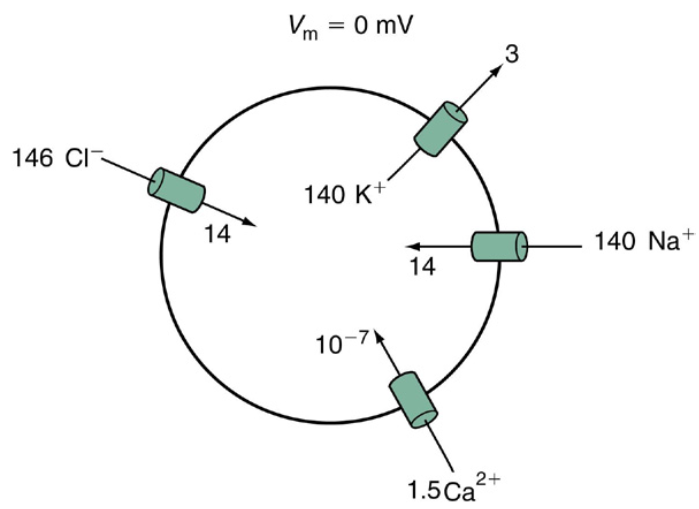
\includegraphics[height=6cm]{Pictures/Anakin/c.grad.png}
  \end{subfigure}
  \hfill
  \begin{subfigure}[t]{0.45\textwidth}
    \centering
    \caption{}\label{sfig:dirB}
    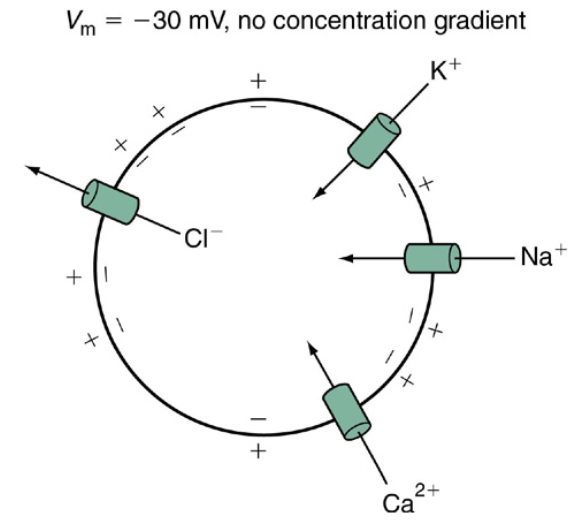
\includegraphics[height=6cm]{Pictures/Anakin/el.grad.png}
  \end{subfigure}
    \caption{Passive diffusion of \glspl{gls:ion}. Passive diffusion of \glspl{gls:ion} according \labelcref{sfig:dirA} their concentration \gls{gls:grad} only, or \labelcref{sfig:dirB} to \gls{gls:membrane} \gls{gls:Pote} (electrical \gls{gls:grad}) only \(\br{\unit{\V\membrane} = \qty{-30}{\mV}}\). From \cite{Hammond2015ch3}}\label{fig:direction} 
\end{figure}


\subsection{Ionic currents}
The passive diffusion of \glspl{gls:ion} through an open channel is a movement of charge through a resistance (resistance here is a measure of the difficulty of \glspl{gls:ion} moving through the channel pore). Movement of charges through a resistance is a current. Through a single channel the current is called `single-channel current' or `unitary current', \(\br{\ucur\ion}\). The amplitude of \(\ucur\ion\) is expressed in ampere \(\br{\unit{\ampere}}\) which are coulombs per seconds \(\br{\unit{\coulomb\per\second}}\). 

In general, currents are expressed following ohm's law: \(\rmm{U}=\rmm{R}\curr\), where \(\curr\) is the current through a resistance \(\rmm{R}\) and \(\rmm{U}\) is the difference of \gls{gls:Pote} between the two ends of the resistance. 
For currents carried by \glspl{gls:ion} (and not by electrons as in copper wires), \(\curr\) is called \(\curr\ion\), the current that passes through the resistance of the channel pore which has a resistance R \(\br{\res\ion}\). But what is \(\rmm{U}\) in biological systems? 
\unit{U} is the force that makes \glspl{gls:ion} move in a particular direction; it is the electrochemical \gls{gls:grad} for the considered \gls{gls:ion} and is also called the driving force: \(\rmm{U}=(\unit{\V} - \equi\ion)\). According to ohm's law, the current \(\curr\ion\) through a single channel is derived from 
\begin{equation}
  \unit{\V} - \equi\ion = r\ion \cdot \curr\ion
\end{equation}
So:
\begin{equation}\label{eq:cur2con}
  \curr\ion= \frac{1}{r\ion\br{\unit{\V} - \equi\ion}} = \ucon\ion(\unit{\V\membrane} - \equi\ion)
\end{equation}
\(\ucon\ion\) is the reciprocal of resistance; it is called the \textit{\gls{gls:contan}} of the channel, or unitary \gls{gls:contan}. It is a measure of the ease of flow of \glspl{gls:ion} (flow of current) through the channel pore. Whereas resistance is expressed in \gls{gls:ohm} \(\br{\unit{\ohm}}\), \gls{gls:contan} is expressed in siemens \(\br{\unit{\siemens}}\). By convention \(\curr\ion\) is negative when it represents an inward \gls{gls:flux} of positive charges (\glspl{gls:cation}) and \(\curr\ion\) is positive when it represents an outward \gls{gls:flux} of positive charges. It is generally of the order of pico-ampere \(\br{\qty{1}{\pico\ampere}=\qty{e-12}{\ampere}}\). At physiological concentrations, \(\ucon\ion\) varies between \(\qtyrange{10}{150}{\pico\siemens}\) dependent on channel type~\cite{Hammond2015ch4}.

\(\curr\ion\) and \(\ucur\ion\) can be measured experimentally. The former is measured current from a patch of \gls{gls:membrane} where only one channel of a given type is present. \(\curr\ion\) is current measured from a whole \gls{gls:membrane} where \(N\) channels of the same type are present. The techniques mainly used for measuring ionic currents in excitable cells are the current clamp and voltage clamp techniques.

\subsubsection{Current clamp}\label{sec:Cclamp}

The current clamp mode is a technique for recording the membrane potential and its changes by injecting current into a cell through the recording electrode.  "Current clamp" implies that the current applied through the electrode is held at a constant value by the experimenter, while the membrane potential is free to vary, and the amplifier records whatever voltage the cell generates on its own or as a result of stimulation. This technique is useful for studying how a cell responds when electric current enters a cell~\cite{Hammond2015ch4}.

\subsubsection{Voltage clamp technique}\label{sec:Vclamp}
 
In contrast to the current clamp technique, in voltage clamp mode the cell potential is ``clamped'' at a chosen value while recording changes in ion currents. This allows to measure how much \textit{ionic current} flows through the cell's membrane at any given voltage. This is important because, as will be elaborated in the following sections, many of the ion channels in neuronal membrane are \gls{gls:vgate}[d] ion channels, which open only when the membrane voltage is within a certain range, and the voltage clamp technique allows for control of the variable determining the opening of those channels~\cite{Hammond2015ch4}.

A variation of  voltage clamp technique is the patch clamp technique, which allows to isolate currents from patches of cell membrane or even individual ion channels (unitary currents \(\ucur\ion\))~\cite{Hammond2015ch4}.

\subsection{Equilibrium Potential of a Given Ion}
\begingroup
\allowdisplaybreaks
All systems yearn for their \gls{gls:equil}, the fabled \textit{steady state}. This divine relation of the components in a system, one achieved, the system no longer needs to evolve, it has been perfected by entropy. 
The value of the \gls{gls:mPote} is constantly fluctuating depending on the relative distribution of charged particles that cross the \gls{gls:membrane}. The relationship can be illustrated as the relative `work' \(\br{W}\) of concentrations, where  \(\br{W_c}\) represents the force moving against the electrical gradient done by the concentration gradient, and \(\br{W_e}\) is the force of the electrical gradient against concentration. The equilibrium exists at;
\begin{equation}
    W_e + W_c = 0
\end{equation}
%The \gls{gls:ePote} for a particular \gls{gls:ion} is the value of \(\unit{\V\membrane}\) for which the net \gls{gls:flux} of this \gls{gls:ion}\(\br{f_\bfm{net}}\) through an open channel is null: when \(\unit{\V\membrane} = \equi\ion\), \(f_\bfm{net} = \qty{0}{\mole\per\second}\).
When the direction of the \gls{gls:grad} is perfectly balanced at net zero, it is referred to as the `\gls{gls:ePote}' of the given \gls{gls:ion} \br{\equi\ion}, alternatively, as the `\gls{gls:rPote}' of the \gls{gls:ion} \(\equi\reverse\). 
The \(\equi\ion\) of the given \glspl{gls:ion} can be calculated using the \emph{Nernst} equation for equilibrium potential of an ion species:
\begin{subequations}\label{eq:nernst}
\begin{equation}
  \equi\ion = \br{\frac{\clm{R}\, \cdot \,\clm{T}}{z\, \cdot \, \clm{F}}} \, \ln \br{\frac{\ionconc\excell }{ \ionconc\incell} } \tag{\ref*{eq:nernst}} 
\end{equation}

Where \(\clm{R}\) is the ideal gas constant \br{\qty{8.314}{\cubic\meter\pascal\per\kelvin\per\mol}}; \(\clm{T}\) is the temperature in \gls{gls:kelvin} \(\br{ x\,\unit{\glssymbol{gls:celsius}} \cong {273.15} + x\,\unit{\kelvin}}\); \(\clm{F}\) is the Faraday constant \br{\qty{96500}{\coulomb\per\mole}}; \(z\) is the valence of the \gls{gls:ion}; and \(\ionconc\) is the concentration of the given \gls{gls:ion} in the \gls{gls:excell} \( \br{ \clm{E} } \) or \gls{gls:incell} \( \br{\clm{I}}\) \gls{gls:media}. 
As most of these terms are constants, it is simple to reduce the equation down in dimensional complexity:
\begin{align} 
    \equi\ion &= \br{\frac{ \qty{8.314}{\cubic\meter\pascal\per\mol\per\kelvin} \, \cdot \, \clm{T}}{ z\, \cdot \, \qty{96500}{\coulomb\per\mole} }} \,\ln \br{ \frac{ {\ionconc\excell} }{ {\ionconc\incell}} } \\
    %\equi\ion &= \br{\frac{ {8.314} \cdot \(t\) \cdot \unit{\cubic\meter\pascal} \,\cancel{\unit{\per\mol}}\,\cancel{\unit{\per\kelvin\kelvin}} }{ z\, \cdot \, \qty{96500}{\coulomb} \,\cancel{\unit{\per\mol}}}} \,\ln \br{ \frac{ {\ionconc\excell} }{ {\ionconc\incell}} } \\
    %
    %\equi\ion &= \br{\frac{ {8.314} \, \cdot \, \(t\) \, \unit{\cubic\meter\pascal} }{ z\, \cdot \, \qty{96500}{\coulomb}} } \,\ln \br{ \frac{ {\ionconc\excell} }{ {\ionconc\incell}} } \\
    %
    \intertext{dividing and rearranging the terms:}
    \equi\ion &= \br{\frac{ \clm{T}\unit{\per\K} \, \unit{\cubic\meter\pascal} }{ z\, \cdot \, \qty{11612.515042118}{\coulomb} } } \cdot \,\ln \br{ \frac{ {\ionconc\excell} }{ {\ionconc\incell}} } \\
    %
    \intertext{converting the unit of pressure, pascal \br{\unit{\pascal}} to the base units representing mass over an area over time \br{\unit{\kilo\gram\per\meter\per\square\second}}, as well converting the unit for charge, a \gls{gls:coulomb} \br{\unit{\coulomb}}, to the base units denoting the quantity of current in a second, \br{\unit{\ampere\second}}, gives the substitution:}
    \equi\ion &= \br{\frac{ \clm{T}\unit{\per\K} \, \unit{\cubic\meter\kilo\gram\per\meter\per\square\second} }{ z\, \cdot \, \qty{11612.515042118}{\ampere\second} } } \cdot \,\ln \br{ \frac{ {\ionconc\excell} }{ {\ionconc\incell}} } \\
    %\intertext{at this point we're only left with base SI units, so we need to be a little silly, the unit of magnetic \gls{gls:flux} is defined \(\unit{\weber} = \unit{\kilo\gram\square\meter\per\square\second\per\ampere}\), implying through substitution \(\unit{\kilo\gram\square\meter\per\cubic\second\per\ampere} = \unit{\weber\per\second} \):}
    %\equi\ion &= \frac{ \clm{T}\unit{\per\K} }{ z\, \cdot \, \num{11612.515042118}} \cdot \br{\unit{\weber\per\second}} \cdot \,\ln \br{ \frac{ {\ionconc\excell} }{ {\ionconc\incell}} } \\
    %
    \intertext{a unit describing the rate of change of magnetic charge per second, which is equivalent to a Volt, \(\unit{\weber\per\second} = \unit{\volt} = \unit{\kilo\gram\square\meter\per\cubic\second\per\ampere} \), the combination of units found through deconstruction is the literal base unit definition of a volt:}
    \equi\ion &= \frac{ \clm{T}\unit{\per\K} }{ z\, \cdot \, \num{11612.515042118}} \cdot \unit{\volt} \cdot \ln \br{ \frac{ {\ionconc\excell} }{ {\ionconc\incell}} }\label{eq:derivedNerst}
    %\equi\ion &= \cfrac{ \(t\) \cdot \,\ln \br{ \cfrac{\ionconc\excell }{ \ionconc\incell} } }{ z\, \cdot \, \num{11612.515042118}} \cdot \unit{\volt} \cdot \qty{1000}{\milli\volt\per\volt} \\
    %\equi\ion &= \cfrac{ \(t\) \cdot \,\ln \br{ \cfrac{\ionconc\excell }{ \ionconc\incell} } }{ z\, \cdot \, 1 \, 160} \ \unit{\milli\volt}
\end{align}
%{Volume Concentration \per\kelvin\per\mol}
%{\kilo\gram\metre^2\second^{-2}\kelvin\per\mol}
\end{subequations}

\begin{subequations}\label{eq:mVions}
With minor adjustments to \cref{eq:derivedNerst}, the now derived form of \cref{eq:nernst}, one is able to get
\begin{equation}
  \equi\ion = \cfrac{\clm{T}\unit{\per\K}}{ z } \, \cdot \, \ln \br{ \frac{ {\ionconc\excell} }{ {\ionconc\incell}} } \cdot \num{11.612515042}^{-1} \ \unit{\milli\volt} \tag{\ref*{eq:mVions}}
\end{equation}

Plugging the relative concentrations, measured in millimols \br{\unit{\milli\mol}}, of each \gls{gls:ion} into \cref{eq:mVions}, as well as choosing an arbitrary temperature, such as human body temperature \(\approx\) \qty{37}{\degreeCelsius} \(\br{\sbr{\num{37} + \num{273.15}}\unit{\glssymbol{gls:kelvin}}}\),
using the relevant \(\ionconc\),
the \glspl{gls:ePote} follow:
\begin{minipage}{.48\textwidth}
  \begin{align}
    {\equi\sodium} &= \num{310.15}\ \ln \br{ \frac{142}{15} }\cdot \num{11.612515042}^{-1} = \qty{60.034194963}{\mV} \label{eq:Na}\\
    {\equi\potassium}  &= \num{310.15}\ \ln \br{ \frac{4}{150} }\cdot \num{11.612515042}^{-1} = \qty{-96.799817808}{\mV} \label{eq:K}
  \end{align}
\end{minipage}
~
\begin{minipage}{.48\textwidth}
  \begin{align}
    {\equi\chlorine}  &= \num{-310.15}\ \ln \br{ \frac{120}{\num{5}} }\cdot \num{11.612515042}^{-1} = \qty{-90.840043187}{\mV} \label{eq:Cl}\\
    {\equi\calcium}  &= \frac{310.15}{2}\ \ln \br{ \frac{1}{\num{e-4}} }\cdot \num{11.612515042}^{-1} = \qty{122.996054517}{\mV} \label{eq:Ca}
  \end{align}
\end{minipage}

% 293.15

% 58.127185848 
% -97.014667339
% 121.372216367
% -59.186543354

\end{subequations}

% These equations can be interpreted such that when
% \gls{K} channels open in the \gls{gls:membrane}, the efflux of \gls{K} \glspl{gls:ion} will hyper-polarize the \gls{gls:membrane} until \(\unit{\V\membrane} = \equi\potassium \approx \qty{-97}{\mV}\), at which point the net \gls{gls:flux} of \gls{K} is null being that \gls{K} \glspl{gls:ion} have exactly the same \gls{gls:Pote} to move towards the \gls{gls:excell} space as the \gls{gls:incell} space. 
% The efflux of \gls{K} will be exactly compensated by the influx of \gls{K} and the \gls{gls:mPote} will stabilize at \(\equi\potassium\) for as long as the \gls{K} channels stay open. 
% Assuming only \gls{Na} channels are open, the \gls{gls:mPote} will move toward \(\unit{\V\membrane} = \qty{58}{\mV}\), the \gls{gls:Pote} at which the net \gls{gls:flux} of \gls{Na} is null. 
% Similarly, when \(\unit{\V\membrane} = \equi\chlorine \approx \qty{-59}{\mV}\), 
% %\gls{Cl} \glspl{gls:ion} have the tendency to move down their concentration \gls{gls:grad} than to move in the reverse direction according to \gls{gls:mPote}, 
% the net \gls{gls:flux} of \gls{Cl} is null. 
% By extension, should \(\unit{\V\membrane} \neq \equi\potassium\), the net \gls{gls:flux} of \gls{K} will no longer be null. 
% This holds true for all \glspl{gls:ion}: when \(\unit{\V\membrane} \neq \equi\ion\) there is a net \gls{gls:flux} of the \gls{gls:ion}~\cite{Hammond2015ch4}. The difference \(\br{\unit{\V\membrane} - \equi\ion}\) is called the electrochemical \gls{gls:grad}. It is the force that makes the \glspl{gls:ion} move through an open channel.


%The membrane potential never gets as high as vNa, therefore sodium will flow into the cell whenever sodium channels are open. 

\endgroup

\section{Action Potential}\label{sec:ap}
Functionally all eukaryotic \glspl{gls:membrane} maintain a difference in voltage between the \gls{gls:excell} and \gls{gls:incell} space, this difference is called the `\gls{gls:mPote}'. The expected \gls{gls:mPote} in human cells is \glslink{gls:volt}{\qty{-70}{\milli\volt}}~\cite{}.
\gls{ap} is the measure of the \gls{gls:Pote} that causes action.

An \gls{ap} occurs when the \gls{gls:Pote} of an excitable cell's \gls{gls:membrane} rapidly rises and falls. This \gls{gls:depol} then causes adjacent regions to similarly `depolarize', creating a chain reaction in the form of a `wavelet'.
The voltage fluctuations take the form of a rapid upward spike followed by a rapid fall.

%``All-or-none'' principle

\begin{figure}[H]
  \centering
  \import{../../Pictures/Anakin}{Channels.tex}
  \caption{ $\langle \text{temp} \rangle$ }\label{fig:Channels}
\end{figure}

\begin{comment}
  Each excitable patch of \gls{gls:membrane} has two important levels of \gls{gls:mPote}: the resting potential, which is the value the \gls{gls:mPote} maintains as long as nothing perturbs the cell, and a higher value called the \gls{gls:tPote}. At the axon hillock of a typical \gls{gls:neuron}, the resting \gls{gls:Pote} is around –70 millivolts (mV) and the threshold \gls{gls:Pote} is around –55 mV. Synaptic inputs to a \gls{gls:neuron} cause the \gls{gls:membrane} to depolarize or hyperpolarize; that is, they cause the \gls{gls:mPote} to rise or fall. \glspl{ap} are triggered when enough \gls{gls:depol} accumulates to bring the \gls{gls:mPote} up to threshold. When an \gls{ap} is triggered, the \gls{gls:mPote} abruptly shoots upward and then equally abruptly shoots back downward, often ending below the resting level, where it remains for some period of time. The shape of the \gls{ap} is stereotyped; this means that the rise and fall usually have approximately the same amplitude and time course for all \glspl{ap} in a given cell. (Exceptions are discussed later in the article). In most \glspl{gls:neuron}, the entire process takes place in about a thousandth of a second. Many types of \glspl{gls:neuron} emit \glspl{ap} constantly at rates of up to 10–100 per second. However, some types are much quieter, and may go for minutes or longer without emitting any \glspl{ap}.

  \glspl{ap} result from the presence in a cell's \gls{gls:membrane} of special types of \gls{gls:vgate}[d] \glspl{gls:ionChan}.[6] A \gls{gls:vgate}[d] \gls{gls:ion}channel is a transmembrane protein that has three key properties:

  It is capable of assuming more than one conformation.
  At least one of the conformations creates a channel through the \gls{gls:membrane} that is permeable to specific types of \glspl{gls:ion}.
  The transition between conformations is influenced by the \gls{gls:mPote}.
  Thus, a \gls{gls:vgate}[d] \gls{gls:ion}channel tends to be open for some values of the \gls{gls:mPote}, and closed for others. In most cases, however, the relationship between \gls{gls:mPote} and channel state is probabilistic and involves a time delay. \Glspl{gls:ionChan} switch between conformations at unpredictable times: The \gls{gls:mPote} determines the rate of transitions and the probability per unit time of each type of transition.
\end{comment}
%original text
The \gls{ap} is a sudden and rapid \gls{gls:depol} of the \gls{gls:membrane} as a result of positive inward \gls{gls:flux} of current through the \gls{gls:axon}. In \gls{gls:neuron}[al] \glspl{gls:soma} and \glspl{gls:axon}, these currents are most commonly propogated by \gls{Na} \glspl{gls:cation}.{}\footnote{A positively charged \gls{gls:ion}, no relation to \textit{Felis Catus}}

The \gls{gls:ion}[ic] basis for \gls{gls:neuron}[al] excitation was first described in the giant squid axon by Hodgkin \& Huxley \br{1952} using the voltage clamp technique~\cite{HodHux1952}. They observed a key phenomenon, that the \gls{ap} is underlied by two separate voltage-dependent currents: an early transient inward \gls{Na} current which depolarizes the \gls{gls:membrane}, and a delayed outward \gls{K} current largely responsible for \gls{gls:repol}. 
The resulting voltage waveform takes the shape of a rapid upward spike followed by a rapid inactivation that hyperpolarizes the \gls{gls:membrane} before returning to the resting \gls{gls:mPote} \Cref{fig:AP}.

Up to a threshold level of \gls{gls:membrane} \gls{gls:depol} (called the \gls{gls:tPote}), only passive ohmic response can be recorded, when the \gls{gls:membrane} is depolarized just above the threshold, an \gls{ap} is evoked. 
Increasing the intensity of the stimulating current pulse does not increase the amplitude of the \gls{ap}, the \gls{ap} is all or none. 
\begin{figure}[H]
  \centering
  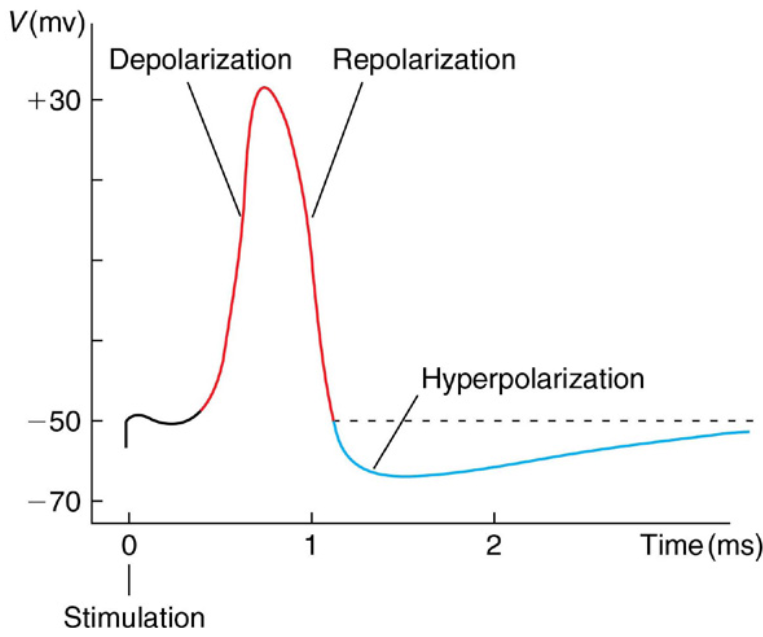
\includegraphics[width=0.5\linewidth]{Pictures//Anakin/AP.png}
  \caption{The action potential spike, indicating the different phases.}\label{fig:AP}
\end{figure}

\subsubsection{Depolarization of the membrane potential}
%\subsubsection{The \gls{gls:depol} phase of \gls{Na}[-dependent] \gls{ap} results from the transient entry of \gls{Na} \glspl{gls:ion} through \gls{gls:vgate}[d] \gls{Na} channels.}
The threshold for initiation of \gls{Na}[-dependent] action \gls{gls:Pote} is due to \gls{gls:vgate}[d] \gls{Na} channels only opening in response to a \gls{gls:depol} of \qtyrange{-50}{-40}{\mV}, hence the classification `\gls{gls:vgate}[d]'. 

In response to \gls{gls:depol} passing the \gls{gls:tPote}, closed \gls{Na} channels of the axon segment begin to open. The \gls{gls:flux} of \gls{Na} \glspl{gls:ion} through the open \gls{Na} channels depolarize the \gls{gls:membrane} more, triggering the opening of additional \gls{Na} channels. 
Consequentially, the \gls{gls:flux} of \gls{Na} \glspl{gls:ion} increases, causing further \gls{gls:depol} of the \gls{gls:membrane}, cascading until all \gls{Na} channels in the segment have opened. 
This coincides with the \gls{gls:depol} phase reaching its peak. 

{}\gls{Na} channels are opened by \gls{gls:depol} and once opened, they reinforce the \gls{gls:membrane} \gls{gls:depol} and therefore their own activation: a self-maintained process,\footnotemark~which is why the \gls{Na}[-dependent] \gls{ap} is all or none.\footnotetext{Also commonly refered to as a `positive feedback cycle'.}
Once initiated, the \gls{ap} propagates along an axon without decaying in amplitude, at rates ranging between \qtyrange{1}{100}{\meter\per\s}. 
This propagation proceeds without \gls{gls:attenuation} due to the density of \gls{gls:vgate}[d] \gls{Na} channels remains constant along the axon; as well due to the presence of insulating \glspl{gls:myelin}. 
Once the channels become inactive, they may not reopen, ensuring that \gls{ap} only propagates forward. 
%originaltextend
The time during which the \gls{Na} channel stays open is the mean open time, denoted \(\tau_o\).\footnote{The letter  `o', not the number `0'}
%The functional significance of this value is the following: during a time equal to \(\tau_o\) the channel has a high probability of staying open. 

The \unit[per-mode = symbol]{\ucur\sodium\per\V} relation is obtained by plotting the amplitude of the unitary current \(\br{\ucur\sodium}\) versus \gls{gls:mPote} \(\br{\unit{\V\membrane}}\). This relation is linear between \qtyrange{-50}{0}{\mV}. For \glspl{gls:mPote} \gls{gls:hypol} beyond \qty{-50}{\mV}, \(\ucur\sodium\) will have close to no value. As illustrated by \cref{eq:Na}, the \gls{Na} channel has a reduced strength of gradient, drastically lowering probability of opening.\footnote{Quantitative data for \glspl{gls:mPote} more depolarized than \qty{0}{\mV} is, \emph{bizarrely}, lacking.}

When the activity of a single \gls{Na} channel is recorded at different test \glspl{gls:Pote}, it was observed that the amplitude of the inward unitary current \(\br{\ucur\sodium}\) diminishes proportionately with the state of \gls{gls:membrane} \gls{gls:depol}~\cite{Hammond2015ch4}. 
The critical point of the current/voltage relation is the \gls{gls:mPote} for which the current is zero; i.e. the \gls{gls:rPote} of the current \(\br{\equi\reverse}\). 
Because exclusively \gls{Na} \glspl{gls:ion} flow through \gls{Na} channels, the \gls{gls:rPote} is equal to \(\equi\sodium\). 
From \qty{-50}{\mV} to \(\equi\reverse\), \(\ucur\sodium\) is inward and its amplitude decreases. This results from the decrease of the \gls{Na} driving force \(\br{\unit{\V\membrane}-\equi\sodium}\) as the \gls{gls:membrane} approaches the \gls{gls:rPote} for \gls{Na} \glspl{gls:ion}. 
For \glspl{gls:membrane} \gls{gls:depol} greater than \(\equi\reverse\), \(\ucur\sodium\) is now outward. Above \(\equi\reverse\), the amplitude of the outward \gls{Na} current progressively increases as the driving force for the exit of \gls{Na} \glspl{gls:ion} increases. 

The relation \unit[per-mode = symbol]{\ucur\sodium\per\V} is \gls{gls:linear}[ly] described by the equation \(\ucur\sodium = \ucon\sodium \br{\unit{\V\membrane}-\equi\sodium}\), where \unit{\V\membrane} is the test potential, \(\equi\sodium\) is the \gls{gls:rPote} of the \gls{Na} current, and \(\ucon\sodium\) is the \gls{gls:contan} of a single \gls{Na} channel (unitary \gls{gls:contan}). The value of \(\ucon\sodium\) is given by the slope of the linear \unit[per-mode = symbol]{\ucur\sodium\per\V} curve. It has a constant value at any given \gls{gls:mPote}. This value varies between \qtyrange{5}{18}{\pico\siemens} depending on the preparation.

\begin{figure}[H]
  \centering
  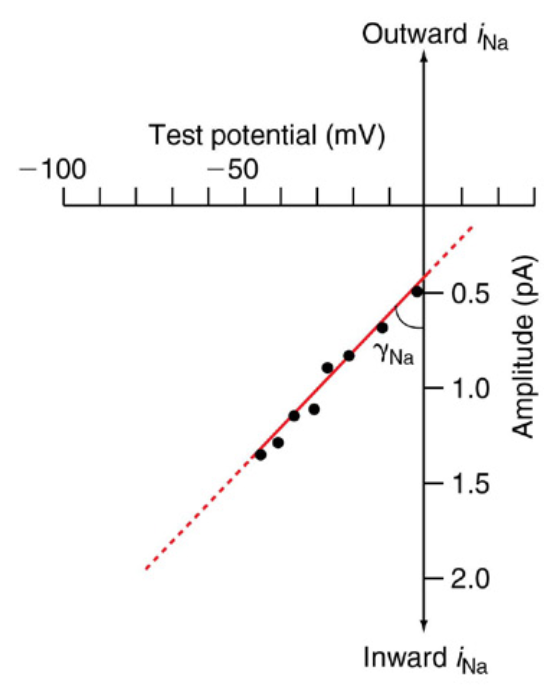
\includegraphics[width=0.5\linewidth]{Pictures//Anakin/iNa-VNa.png}
  \caption{The single-channel current/voltage \br{\unit[per-mode = symbol]{\ucur\sodium\per\volt}} relation is linear. Adapted from Stühmer W, Methfessel C, Sakmann bet al. (1987) patch clamp characterization of sodium channels expressed from rat brain cdNA. Eur. Biophys. J.14, 131–13 }
  \label{fig:NaVNa}
\end{figure}

The probability of \gls{gls:vgate}[d] \gls{Na} channels opening is dependent on voltage and time. 
During cell recordings of \gls{Na} channels, observations showing that when the \gls{gls:mPote} depolarizes, the probability of the \gls{Na} channel being in the open state increases proportional to \gls{gls:depol} until reaching a maximal level~\cite{Hammond2015ch4}. 
The greater the \gls{gls:depol}, the higher is the probability of an individual \gls{Na} channel opening. 
Variation also comes from the time, with greater probability of a channel opening towards the start of \gls{gls:depol}.
Additional observations show that after \qtyrange{4}{6}{\ms}, the probability of the \gls{Na} channel being in the open state decreases drastically~\cite{Hammond2015ch4}. 
Even with a large \gls{gls:depol} step: the \gls{Na} channel inactivates after \qtyrange{4}{6}{\ms}~\cite{Hammond2015ch4}. 
%The probability of the \gls{Na} channel being in the open state at time \(t=\qty{2}{\ms}\), for example, increases with the amplitude of the depolarizing step. To generalize, at \qty{-30}{\mV} the open probability is maximum, and the channels inactivate in \qty{4}{\ms}. 

{}\(\curr\sodium\) is the macroscopic current, or the sum of all unitary currents \(\ucur\sodium\) flowing through all the open \gls{Na} channels of the \gls{gls:membrane} being recorded. Shown in \Cref{fig:unitcurNa}b, an average of \(\num{300}\) unitary \gls{Na} currents elicited by a \gls{gls:depol} pulse of \(\qty{40}{\mV}\). 
For any given potential, the average of inward \gls{gls:flux} for \gls{Na} rises quickly, reaching the peak at time, \(t=\qty{1.5}{\ms}\) \cite{Hammond2015ch4}. 
The peak corresponds to the time when most of the \gls{Na} channels are opened at each trial. 
Subsequently, the average now decays with time because the \gls{Na} channels have a proportionately lower probability of being open.\footnotemark~At each trial, the \gls{Na} channel does not trigger inactivation at exactly the same time, which explains the progressive decay of the average macroscopic \gls{Na} current. 
\footnotetext{Owing to the inactivation of the \gls{Na} channel.}

%The averaged current does not have a rectangular shape because the \gls{Na} channel does not open with the same delay and does not inactivate at the same time at each trial. 

\begin{figure}[H]
  \centering
  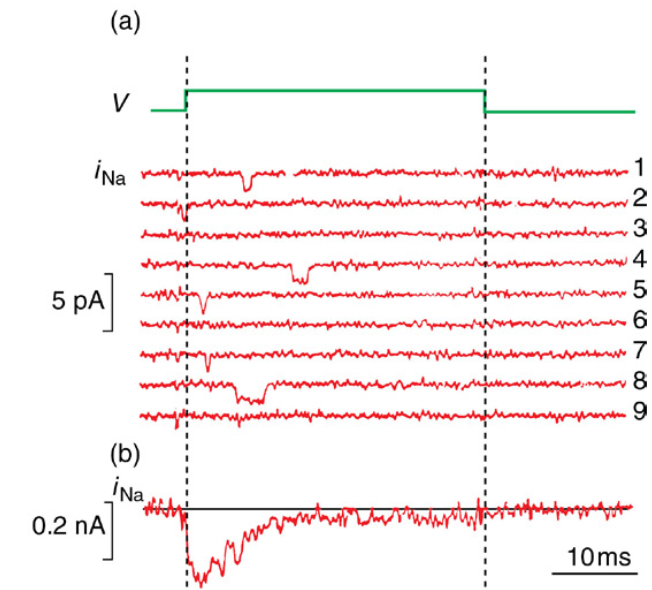
\includegraphics[width=0.5\linewidth]{Pictures//Anakin/iNa.png}
  \caption{Single \gls{Na} channel openings in response to a depolarizing step. (a) Nine successive recordings of single channel openings (\(\ucur\sodium\)) in response to a \qty{ 40}{\mV} depolarizing pulse (V trace in green) applied at 1s intervals from resting \gls{gls:mPote}. (b) Averaged inward \gls{Na} current from 300 elementary \gls{Na} currents as in (a). Adapted from Sigworth FJ, Neher e (1980) Single Na+channel currents observed in rat muscle cells. Nature287, 447–449 }
  \label{fig:unitcurNa}
\end{figure}

The greater the numerical quantity of \gls{Na} channels opened by \gls{gls:depol}, the smoother the current's sum total \gls{Na} will be. 
The value of \(\curr\sodium\) at each time \(t\) at a given \gls{gls:Pote} is: 
\begin{equation}\label{eq:nasum}
  \curr\sodium = p_t \, N \, \ucur\sodium = p_t \sum^N_{n=1} \, \sbr{\ucur\sodium}_n 
\end{equation}
with \(N\) as the total number of \gls{Na} channels in the \gls{gls:membrane} being recorderd and \(p_t\) is the opening probability at time \(t\). 
%\(\ucur\sodium\) is the unitary \gls{Na} current.
%of the \gls{Na} channel; it depends on the \gls{gls:mPote} and on the channel opening and inactivating rate constants. 
%and Np(t) is the number of \gls{Na} channels open at time \(t\). 
Subsequently, the relation of the macroscopic \gls{Na} current \(\curr\sodium\) and voltage \(\unit{\V}\) is not linear, but rather has a recognizable skewed normal distribution, illustrated in \Cref{fig:IVdist}, with a peak at around \qty{-40}{\mV}. 
\begin{figure}[H]
  \centering
  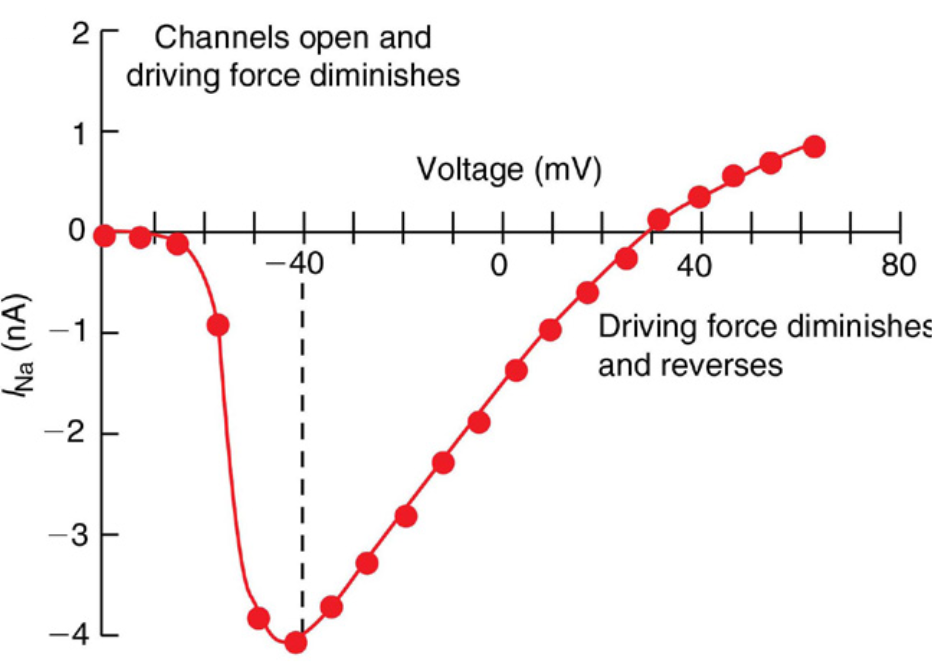
\includegraphics[width=0.5\textwidth]{Pictures//Anakin/I-V.bell.png}
  \caption{The \(\curr\sodium/\unit{\V}\) relation has a bell shape. (From Chiu Sy, ritchie JM, bogart rb, Stagg d (1979) A quantitative description of \gls{gls:membrane} currents from a rabbit myelinated nerve. J. Physiol.292, 149–166)}\label{fig:IVdist}
\end{figure}
 
For small steps, the peak amplitude of current is small, \(\br{\qty{0.2}{\nano\ampere}}\), and has a low peaking rate \(\br{\qty{1}{\milli\second}}\)~\cite{Hammond2015ch4}. At these \glspl{gls:Pote}, the \gls{Na} driving force is strong but the \gls{Na} channels have a low probability of opening. Therefore, \(\curr\sodium\) is small since it represents the current through a small number of open \gls{Na} channels. 

As the depolarizing steps increase in amplitude (\qtyrange{-42}{-35}{\mV}), the amplitude of \(\curr\sodium\) increases to a maximum \(\br{\qty{-3}{\nA}}\) and the time to peak decreases to a minimum \(\br{\qty{0.2}{\ms}}\)~\cite{Hammond2015ch4}. 
Larger \glspl{gls:depol} increase probability of \gls{Na} channels being in the open state and shorten the opening delay. 
Therefore, though the amplitude of \(\ucur\sodium\) decreases by \qtyrange{-63}{-35}{\mV}, the amplitude of \(\curr\sodium\) increases, as a consequence of the increasing quantity of open \gls{Na} channels. 

After the peak, the amplitude of \(\curr\sodium\) decreases to zero, past the peak the probability of opening is no longer enough to compensate for the decrease of \(\ucur\sodium\). 
The \gls{gls:rPote} of \(\curr\sodium\) is the same as that of \(\ucur\sodium\), depending only on the \gls{gls:excell} and \gls{gls:incell} concentrations of \gls{Na} \glspl{gls:ion}.

%\(\curr\sodium\) changes polarity for \unit{\V\membrane} more depolarized than Erev: it is now an outward current whose amplitude increases with the \gls{gls:depol} 

\subsubsection{Activation and inactivation curves}
The `activation rate' is the rate at which macroscopic current flows in response to a \gls{gls:depol} step. 
The \gls{Na} current is recorded in voltage clamp mode~\cite{Hammond2015ch4}.\footnote{see \Cref{sec:Vclamp}}~Depolarizing steps from \qtyrange{-70}{20}{\mV} are applied from a holding \gls{gls:Pote} of \qty{-80}{\mV}. When the ratio of the peak current at each test \gls{gls:Pote} is compared against the maximal peak current \(\br{\curr\sodium/\curr\sodium{\,}_{max}}\); the activation curve of \(\curr\sodium\) can be visualized \cref{fig:actinact}. 
%The distribution is fitted, unsurprisingly, by a sigmoidal curve consistent with logistic growth. 
%In this preparation, the ceiling of \gls{Na} channel activation was measured at \qty{-60}{\mV}. Yet, already at \qty{-40}{\mV}, \(\curr\sodium\) reaches a peak, \(\curr\sodium/\curr\sodium{\,}_{max} = 1\). 
This steepness of activation is characteristic of \gls{gls:vgate}[d] \gls{Na} channels. 

An `inactivation rate', comes as a result of a current decaying during a maintained \gls{gls:depol}. 
%To study inactivation, the \gls{gls:membrane} is held at varying \glspl{gls:Pote} and a fixed \gls{gls:depol} value is applied where \(\curr\sodium\) is maximal (\qty{0}{\mV}, for example). 
The amplitude of \gls{Na} current plotted against the holding \gls{gls:Pote}, shows that \(\curr\sodium\) begins to inactivate at \qty{-90}{\mV} and is fully inactivated at \qty{-50}{\mV}~\cite{Hammond2015ch4}. 
%Taking account that the resting \gls{gls:mPote} in this preparation is around \qty{-80}{\mV}, some of the \gls{Na} channels are already inactivated at rest. 
\begin{figure}[H]
  \centering
  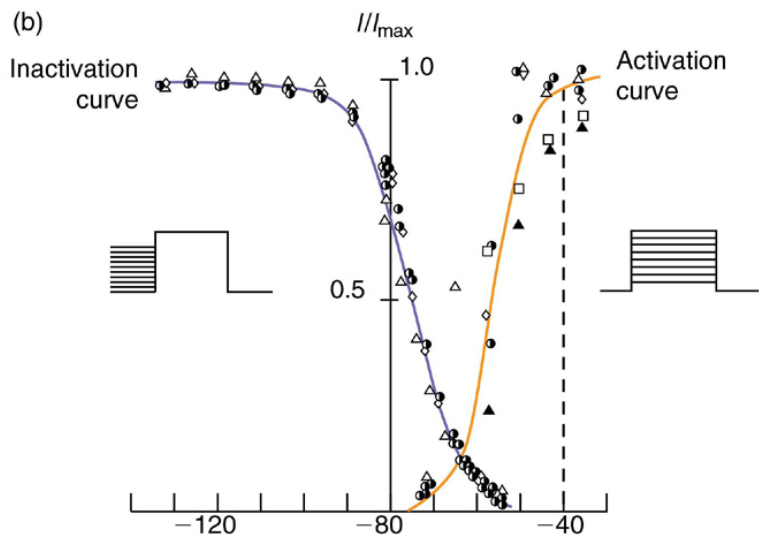
\includegraphics[width=0.5\linewidth]{Pictures//Anakin/activ-inactiv.png}
  %\caption{Activation (right curve) and inactivation (left curve) curves obtained from nine different experiments. The voltage protocols used are shown in insets. In the ordinates, I/Imax represents the ratio of the peak \gls{Na} current (I) recorded at the tested \gls{gls:Pote} of the abscissae and the maximal peak \gls{Na} current (Imax) recorded in this experiment. (From Chiu Sy, ritchie JM, bogart rb, Stagg d (1979) A quantitative description of \gls{gls:membrane} currents from a rabbit myelinated nerve. J. Physiol.292, 149–166) }\label{fig:actinact}
  \caption{}\label{fig:actinact}
\end{figure}

\subsection{Repolarization the membrane potential}
%\subsection{The \gls{gls:repol} phase of the \gls{Na}[-dependent] \gls{ap} results from \gls{Na} channel inactivation and partly from \gls{K} channel activation}

The \gls{gls:repol} phase of the \gls{Na}[-dependent] \gls{ap} results from \gls{Na} channel inactivation and partly from \gls{K} channel activation. The \gls{gls:vgate}[d] channels that participate in \gls{gls:membrane} \gls{gls:repol} are so called `delayed rectifiers', which activate after a delay following the \gls{gls:membrane} \gls{gls:depol} and have a low inactivate rate~\cite{Hammond2015ch4}. The function of delayed rectifier channels is the transduction of \gls{gls:membrane} \gls{gls:depol} into an outward \gls{gls:flux} of \gls{K} \glspl{gls:ion}. 

% The gating behavior of the delayed rectifier channel is different from that of the \gls{Na} channel. Whereas all four voltage-sensitive domains in \gls{K} channels must be activated in order for pore opening to occur, \gls{Na} channel pore opening requires activation of only three voltage-sensitive domains. 
% Thus, part of the difference in activation speed between \gls{Na} and \gls{K} channels may be due to the lesser number of voltage-sensitive domains required to move in \gls{Na} channels.

The mean open time, \(\tau_o\), measured in the clamped patch is \qty{4.6}{\ms}. While the mean closed time, \(\tau_c\), is \qty{1.5}{\ms}, illustrated by \Cref{fig:Kchannel}. As seen in the figure, during a \gls{gls:depol} to \qty{0}{\mV} the delayed rectifier channels spend a greater time in the open state, compared to the closed state: at \qty{0}{\mV} the average probability of channels being open is relatively high \(\br{p_o = 0.76}\)~\cite{Hammond2015ch4}.

% In order to test whether the delayed rectifier channels show some inactivation, long-lasting recordings are performed. 
% Though no significant inactivation is apparent during test pulses in the range of seconds, during long test \glspl{gls:depol} (in the range of minutes) the channel shows steady-state inactivation at positive holding \glspl{gls:Pote} (not shown). 
% Therefore, in the range of seconds, the inactivation of the delayed rectifier channel can be omitted: the channel fluctuates between the closed and open states:
% \[C\rightleftharpoons O\]
% The transition from the closed (C) state to the open (O) state is triggered by \gls{gls:membrane} \gls{gls:depol} with a delay. 
Delayed rectifiers activate over the range of milliseconds. By contrast, the \gls{Na} channels activate in a range of sub-milliseconds. 
During \gls{gls:membrane} \gls{gls:depol} and \gls{gls:repol}, the \gls{Na} channels will frequently transition between \gls{o} and \gls{c} states. 
\begin{figure}[H]
    \centering
    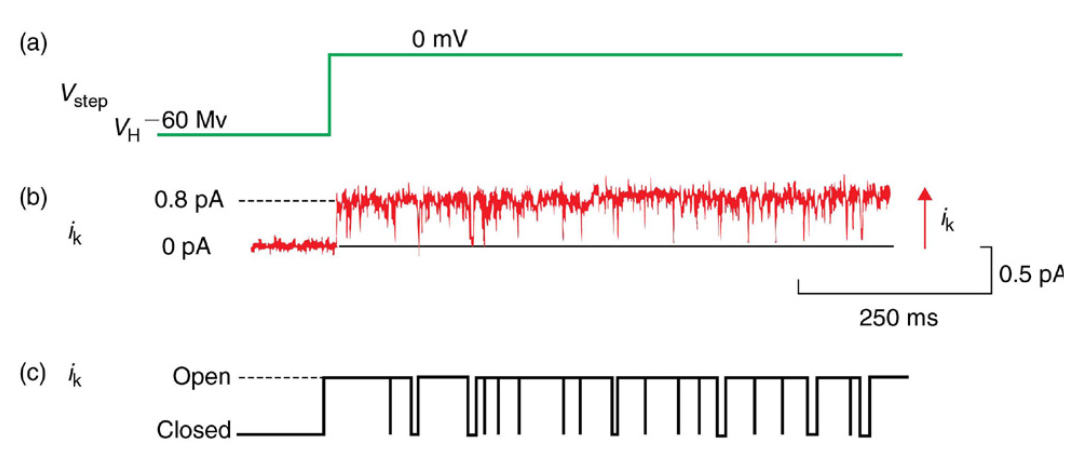
\includegraphics[width=0.8\linewidth]{Pictures//Anakin/Kchannel.png}
    %\caption{Single \gls{K} channel openings in response to a depolarizing step. The activity of a single delayed rectifier channel expressed from rat brain is recorded in patch clamp (inside-out patch). A depolarizing step to \qty{0}{\mV} from a holding \gls{gls:Pote} of \qty{-60}{\mV}(a) evokes the opening of the channel (b). The elementary current is outward. The channel then closes briefly and reopens several times during the \gls{gls:depol}, as shown in the drawing (c) that interprets the current trace. Adapted from Stühmer W, Stocker M, Sakmann bet al. (1988) potassium channels expressed from rat brain cdNA have delayed rectifier properties. FEBS Lett.242, 199–206, with permission. }\label{fig:rangeThree}
    \caption{}\label{fig:Kchannel}
 \end{figure}

The \gls{K} channel has a constant unitary \gls{gls:contan} \(\br{\ucon\potassium}\). In \Cref{fig:rangeThree}a, unitary \gls{K} currents are shown responding to increasing \gls{gls:depol} of \qtyrange{-50}{20}{\mV} from the holding \gls{gls:Pote} of \qty{-80}{\mV}. 
It can be observed that both the amplitude of \(\ucur\potassium\) and the time spent by the channel in the open state increase with \gls{gls:depol}. 

When the mean amplitude of the unitary \gls{K} current is plotted versus \gls{gls:membrane} test potential, a linear \(\ucur\potassium/\unit{\V}\) relation is obtained. This linear \(\ucur\potassium/\unit{\V}\) relation (between \qtyrange{-50}{20}{\mV}) is described by the equation \(\ucur\potassium = \ucon\potassium(\unit{\V\membrane}-\equi\potassium)\), where \unit{\V\membrane} is the \gls{gls:mPote}, \(\equi\potassium\) is the \gls{gls:rPote} of the \gls{K} current, and \(\ucon\potassium\) is the \gls{gls:contan} of the single delayed rectifier \gls{K} channel, which defines the unitary \gls{gls:contan}. 

%Linear back-extrapolation gives a \gls{gls:rPote} value around \qtyrange{-90}{-80}{\mV}, a value close to \(\equi\potassium\) calculated from the Nernst equation. This means that from \qty{-80}{\mV} to more depolarized \glspl{gls:Pote}, which correspond to the physiological conditions, the \gls{K} current is outward. For more \gls{gls:hypol} \glspl{gls:Pote}, the \gls{K} current is inward. The value of \(\ucon\potassium\) is given by the slope of the linear \(\ucur\potassium/V\)curve. It has a constant value at any given \gls{gls:mPote}. This value varies from \qtyrange{10}{15}{\pico\siemens} depending on the preparation. 

\begin{figure}[H]
   \centering
   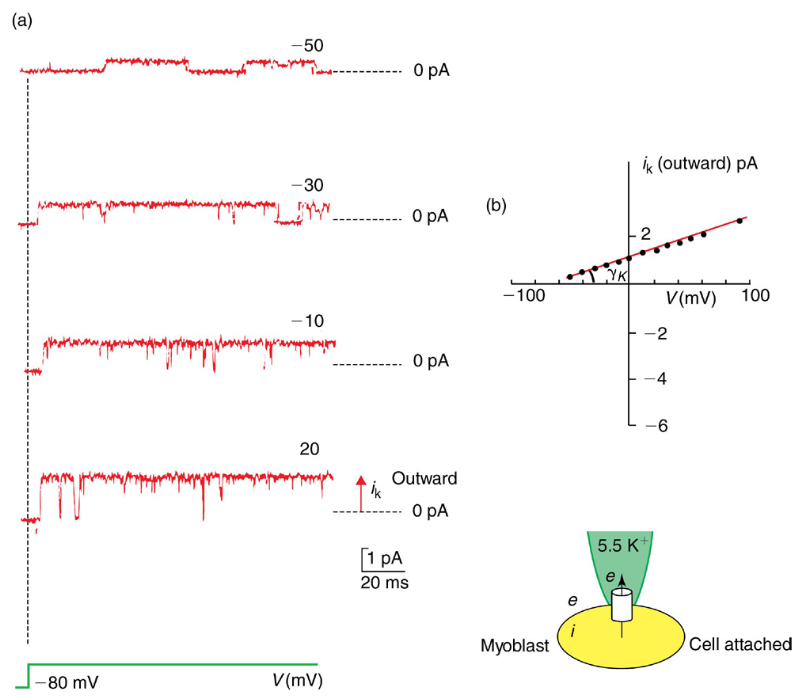
\includegraphics[width=0.8\textwidth]{Pictures//Anakin/I-V.K.png}
   %\caption{The single-channel current/voltage (\(\ucur\potassium\)/V) relation is linear.delayed rectifier \gls{K} channels from rat brain are expressed in a myoblast cell line. (a) The activity of a single channel is recorded in patch clamp (cell-attached patch). Unitary currents are recorded at different test \glspl{gls:Pote} (from \qty{-50}{\mV} to \qty{20}{\mV}) from a holding \gls{gls:Pote} at \qty{-80}{\mV}. Bottom trace is the voltage trace. (b)\(\ucur\potassium\)-V relation obtained by plotting the mean amplitude of \(\ucur\potassium\) at the different test \glspl{gls:Pote} tested. \(\ucur\potassium\) reverses at =\qty{-75}{\mV} and gK=14pS. Adapted from Koren G, liman er, logothetis deet al. (1990) Gating mechanism of a cloned potassium channel expressed in frog oocytes and mammalian cells. Neuron2, 39–51.}\label{fig:rangeThree}
   \caption{}\label{fig:rangeThree}
 \end{figure} 

The macroscopic delayed rectifier \gls{K}current \(\br{\curr\potassium}\) has a delayed voltage dependence of activation and inactivates within tens of seconds. 
%Whole cell currents start to activate at \glspl{gls:Pote} positive to \qty{-30}{\mV} and their amplitude is clearly voltage dependent. 
%When unitary currents recorded from 70 successive depolarizing steps to \qty{0}{\mV} are averaged (Figure4.20b), the macroscopic outward current obtained has a slow time to peak \(\br{\qty{4}{\ms}}\) and lasts the entire depolarizing step. 
The whole cell current amplitude at steady-state for a given \gls{gls:Pote} is:
\begin{equation}\label{eq:ksum}
    \curr\potassium = N p_o \ucur\potassium = p_o \sum^N_{n=1} \, \sbr{\ucur\potassium}_n 
\end{equation}

where \(N\) is the number of delayed rectifier channels in the \gls{gls:membrane} recorded, \(p_o\) the open probability at steady state and \(\ucur\potassium\) the elementary current. The number of open channels \(N\,p_o\) increases with \gls{gls:depol} (to a maximal value) and so does \(\curr\potassium\). 

The \(\curr\potassium/\unit{\V}\) relation shows that the whole cell current varies linearly with voltage from a threshold \gls{gls:Pote} which, for those conditions, is around \qty{-40}{\mV}. When the \gls{gls:membrane} is more \gls{gls:hypol} than the \gls{gls:tPote}, very few channels are open and \(\curr\potassium\) is equal to zero. For \glspl{gls:mPote} more depolarized than the \gls{gls:tPote}, \(\curr\potassium\) depends on \(p_o\) and the driving force state (V-EK) which augments with \gls{gls:depol}. once \(p_o\) is maximal, \(\curr\potassium\) augments linearly with \gls{gls:depol} since it depends only on the driving force. 

\begin{figure}[H]
  \centering
  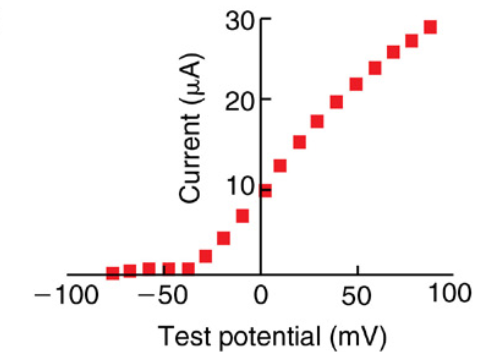
\includegraphics[width=0.4\linewidth]{Pictures//Anakin/IK-V.png}
  %\caption{Characteristics of the macroscopic delayed recti-fier \gls{K} current. The amplitude of the current at steady state is plotted against test \gls{gls:Pote}. The \gls{gls:Pote} threshold for its activation is \qty{-40}{\mV}. From Stühmer W, Stocker M, Sakmann bet al. (1988) potassium channels expressed from rat brain cdNA have delayed rectifier properties. FEBS Lett.242, 199–206. }\label{fig:Kcurrent}
  \caption{}\label{fig:Kcurrent}
\end{figure}

To summerize, %owing to their delay of opening, 
delayed rectifier channels begin to open when the \gls{gls:membrane} is has undergone \gls{gls:depol} by the entry of \gls{Na} \glspl{gls:ion} through open \gls{gls:vgate}[d] \gls{Na} channels. 
Therefore, the exit of \gls{K} \glspl{gls:ion} does not occur at the same time as the entry of \gls{Na} \glspl{gls:ion}. This allows the \gls{gls:membrane} to first depolarize in response to the entry of \gls{Na} \glspl{gls:ion} and then to repolarize as a consequence of the exit of \gls{K} \glspl{gls:ion}.

\begin{figure}[H]
    \centering
    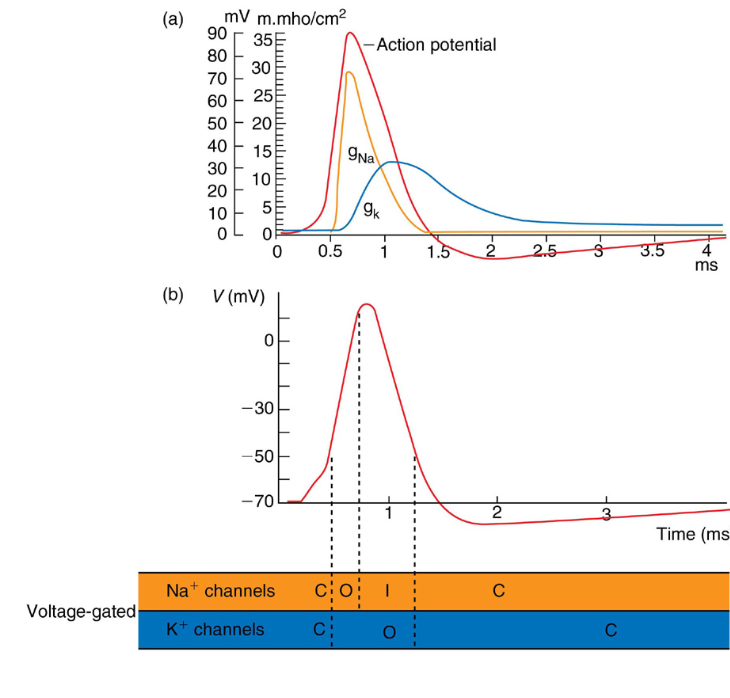
\includegraphics[width=0.8\textwidth]{Pictures//Anakin/N.K.png}
    %\caption{Gating of \gls{Na} and \gls{K} channels during the \gls{Na}[-dependent] \gls{ap}.(a) Interpretation of the manner in which the conductances to \gls{Na} and \gls{K} contribute to the \gls{ap}. (b) State of the \gls{Na} and \gls{K} \gls{gls:vgate}[d] channels during the course of the \gls{ap}. O, channels open; I, channels inactivate; C, channels close or are closed. Trace (a) adapted from Hodgkin Al, Huxley AF (1952) A quantitative description of \gls{gls:membrane} current and its application to conduction and excitation in nerve. J. Physiol.117, 500–544.}\label{fig:Knumber}
    \caption{}\label{fig:Knumber}
\end{figure}



\subsection{Application} 


In physiological conditions, several channels of the same type are open at the same time in the \gls{gls:neuron}[al] \gls{gls:membrane}. 
%Suppose that only one type of channel is open in the \gls{gls:membrane}, for example \gls{Na} channels, the total current \(\curr\sodium\) crossing the \gls{gls:membrane} at time \(t\) is the sum of the unitary currents \(\ucur\sodium\) at time \(t\):
Recall that \Cref{eq:nasum,eq:ksum} gives the relationship of unitary currents to total current for their respective ions, using similarities one can restate the equations 
%(\(N\,p_o\) is therefore the number of open \gls{Na}channels in the \gls{gls:membrane} at time \(t\))
%; and \(\ucur\sodium\) is the unitary \gls{Na} current. \newline
more generally as:
\begin{align}
  \curr\ion&= N \, p_o \, \ucur\ion \label{eq:curgen}\\
\intertext{By analogy, the total \gls{gls:contan} of the \gls{gls:membrane} for a particular \gls{gls:ion} is: }
  \unit{\cond\ion} &= N \, p_o \, \ucon\ion \label{eq:congen}
\intertext{substituting \cref{eq:congen,eq:curgen} into \cref{eq:cur2con} gives us: }
  \curr\ion &= \unit{\cond\ion} \, \br{\unit{\V} - \equi\ion}\label{eq:ionCurrent}
\end{align}

Mr\&Mr hodg-hux did more shit
active/inactive parameters


\end{document}
 